
\section{Introduction}

The Lossy Compression WG was formed in response to \jira{RFC-325} with its charter
being \citedsp{LDM-582}.  In \jira{RFC-325} it was recognized that user 
experience would likely be unacceptably impacted by the long latency required to 
access some LSST image data.  Central to this concern is that the current data model 
does not support storage and serving of processed visit images (PVIs), i.e. the 
detrended, calibrated individual exposures from the survey.  Instead, users needing
such images would either have to rely on retrieval from tape media or regeneration
of the PVIs on-the-fly.

Previous analysis has indicated that retaining all processed images on disk would 
be too costly and therefore not feasible, unless lossy compression is applied. 
The same analysis did indicated that storing all raw data on disk (with a loss-less 
compression) is feasible.  The Lossy Compression WG was asked to investigate whether 
some pipeline products might be saved after applying a lossy compression algorithm 
without significantly degrading their suitability for a wide range of scientific 
investigations.  Central to this is the need that the compressed products be small 
enough that the cost to store and serve these images could be met within a reasonable 
budget.  The benefit from storing compressed products would only be realized if those 
products were indeed useful for many users as it would free resources that otherwise
would be engaged in regenerating or serving a tape archive.

The LSST project has traditionally avoided lossy compression for any of its image data products 
(including the large co-added images as well as templates retained for each data release). 
Anecdotal experience from other recent surveys indicate that science ready images stored
with a lossy compression satisfy the scientific needs of their user communities.  For example, 
the Dark Energy Survey (DES), uses FPACK \citep{PSW2009} with a quantization of 16, 
and Pan-STARRS reportedly uses 4-bits per standard deviation (also equivalent to a 
quantization factor of 16) but with an inverse hyperbolic sine transformation to concentrate 
the sampling near the background level \citep{Wetal2016}.  \citet{Betal2010} have shown that 
for bandwidth limited cases compression reducing images to 2.5-4 bits per pixel using a square-root
compression method would incur only modest loss (effectively 10\% of the observing time) and that 
systematic biases in fluxes and shapes were less than 10$^{-4}$.  Indeed, \citet{PWH2010} have 
argued that none of the scientific information is lost in an astronomical image even with 
fairly drastic quantization (at levels as high as 0.5$\sigma$).  The tests used by \citet{PWH2010} 
were relatively idealized, in this note we describe the results from a small test using 
precursor data from HSC to provide a sense of how lossy compression might be applied for LSST.


\section{Methodology}

This investigation is not meant to address the specific file format(s) that might be
used to store LSST data (e.g.; FITS vs. HDF5).  The tests that have been made were performed
using images stored using FITS, mainly because the changes necessary could be used within 
the current LSST pipeline testing infrastructure.  The specific images used were a set of
HSC data that formed a modest depth patch on which pipeline regression testing was already 
being routinely performed in the development of the LSST pipelines (the {\it ci\_hsc} test set).  
For this test set there were 33 images/CCDs, from 11 visit/exposures, at two bands (HSC-R, HSC-I).
Included among these images are a 4 images near the edge of the HSC focal-plane, where 
vignetting causes a portion of the detector to be unusable for science.  These regions are 
masked and present very different noise characteristics but are useful because they show some 
caveats that must be considered when applying compression.

In this investigation we have separated the loss from the actual compression algorithm.
A change has been injected into the pipeline that allows for a quantization to be applied
to the science (and weight) images that are traditionally stored as floats.  Formally,
the quantization factor, q, determines the number of samples/subdivisions of some set
number, in this case the standard-deviation of the image pixel values that do not contain a 
detected source.  For a FITS image this is expressed as a scale factor (BSCALE) and the image 
pixel values are converted to the nearest integer multiple of this factor.  We then use existing
loss-less compression algorithms to compress the integer representation of the image
to achieve a compressed image.  Our tests varied the factor q from 4 to 128 (stepping by 
factors of 2).  

Metrics are then obtained to understand the impact and efficacy of compression.  Broadly, 
these fall into three categories:
\begin{enumerate}
\item {\bf Image Compression benchmarks:} to measure the changes at the pixel level.  These
include: percent increase in noise/RMS, median difference, and number of pixels that change
by more than the quantization level (to catch cases where the integer representation is not 
able to capture the full dynamic range of the original images).

\item {\bf Catalog/Measurement benchmarks:} to measure the change of aggregate quantities
of interest for scientists using the images for scientific measurements.  The current
benchmarks being measured are source position, flux, and shape along with their associated
uncertainties.

\item {\bf Compression algorithm benchmarks:} to measure the compression factor achieved, along with
algorithm execution times for compression and decompression.
\end{enumerate}
In addition a second set of image and catalog benchmarks are obtained to assess
the changes that might be expected when quantized products are combined to form stacked
images from which astronomical source measurements are also obtained.



\section{Results}

\subsection{Single Image Compression Benchmarks}

At the image level, independent measurements of the noise in the original science 
and weight images (I$_{0}$, W$_{0}$) and the quantized versions (I$_{\rm q}$, W$_{\rm q}$) are made.
The algorithms used are independent of those that performed the estimates used to set the quantization.
In most cases we consider only pixels with FLAG=0 or FLAG=32 (which indicates the presence of a source)
as heavily masked regions often have values (particularly in the weight image) that can exceed the 
range accessible in the quantized images.  

Figure~\ref{pixel_dist} shows the detailed distribution of pixels values for the science and weight planes 
from two images typical of those in the test set.  The first is a typical image, while the second is atypical
in that the image comes from the edge of the HSC focal plane where vignetting and hence significant masking 
occurs.  The difference in the distributions are most apparent in the weights, where it becomes clear that
for the quantization/noise-estimation algorithms to behave consistently, flagged pixels need to be rejected.
A modest amount a caution should be exercised so that image compression acts consistently.  Moreover, it should
noted that flagged data might have very different characteristics after quantization is applied
and their behavior if included in measurements would perform worse than what is seen in the further tests
made in this exercise.  The distributions being considered when determining the quantization factor exclude
all masked pixels (i.e. "mall" and "wmall") but the distributions being analyzed in this work need to understand
the effect on pixels with objects/sources, so we typically include pixels with FLAG=32 (i.e. "mn32" and "wmn32").

Table~\ref{tab_bscale} summarizes the effect of quantization on the original images.  There we include 
the range of BSCALE's (the quantization factor that resulted) for both the science and weight image planes
and then further examine the RMS in the images and examine the fractional increase when comparing the 
measurements on the quantized and un-quantized versions of the image.  The RMS values for the "Original"
images are not the same as that used when setting BSCALE (for the quantization) because RMS values
draw from distributions that include the source pixels (i.e. FLAG=32).  Note that as early as a quantization
factor of q=32, but clearly at q=128, the change in the RMS of the images cannot be well measured 
because the accuracy needed is not available when considering science and weight images comprised 
of 32-bit floats.

\begin{figure}[t]
\centering
  \begin{minipage}{.45\textwidth}
    \centering
    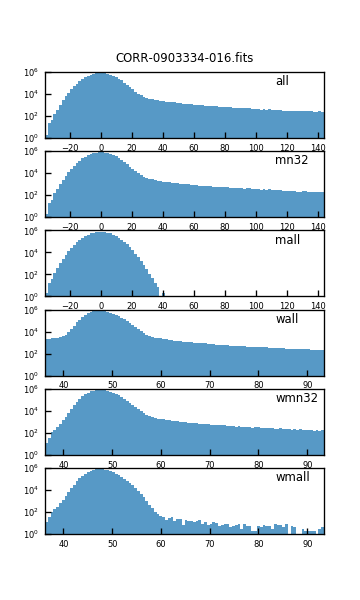
\includegraphics[width=0.9\textwidth]{figure/imgdist_CORR-0903334-016.fits.png}
%    \label{fig:sub1}
  \end{minipage}
  \begin{minipage}{.45\textwidth}
    \centering
    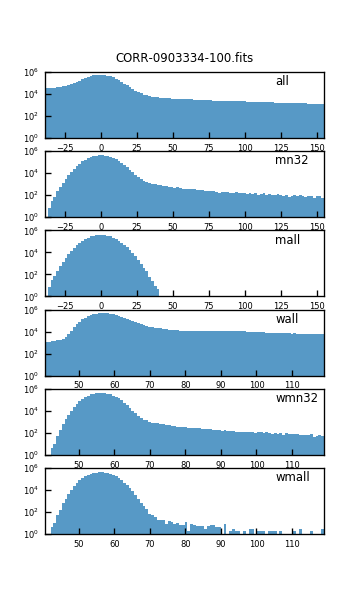
\includegraphics[width=0.9\textwidth]{figure/imgdist_CORR-0903334-100.fits.png}
%   \label{fig:sub2}
  \end{minipage}
\vspace{-32pt}
\caption{Distributions of pixel values from two images in the test set. The left panels show 
distributions from a ``normal image'', while the right panels are for an image near the edge 
of the focal plane with heavy masking.  (top) to (bottom) the panels show: all science plane pixels (all), 
all science pixels with MASK=0 or 32 (mn23), and all unmasked pixels (mall), followed by similar
distributions for the weight plane (wall, wmn32, and wmall).  The "mall" and "wmall" are roughly
the distribution used to estimate the quantization level while "mn32" and "wmn32" are those used
when considering the difference due to quantization.}
\label{pixel_dist}
\end{figure}

\begin{table}
\caption{Summary of BSCALE Values that Resulted in this Test}
\footnotesize
\centering
\begin{tabular}[]{c|cccc|cccc}
\hline
        &  \multicolumn{4}{c}{Science Plane} & \multicolumn{4}{c}{Weight Plane} \\
        &   Min--Max & Median & Median & \% RMS  & Min-Max & Median & Median &  \% RMS \\
 q      &    BSCALE  & BSCALE &  RMS   & Growth  &  BSCALE & BSCALE & RMS    &  Growth \\
\hline
\multicolumn{9}{c}{Sample 1 (HSC-R images)}  \\
\hline
Original &             &       & 7.281  &         &              &       & 2.327 &          \\
    4   & 1.665--2.056 & 1.851 & 7.298  & 0.229 & 0.368--0.977 & 0.605 & 2.337 & 0.417  \\
    8   & 0.832--1.028 & 0.926 & 7.294  & 0.175 & 0.184--0.489 & 0.303 & 2.336 & 0.374  \\
   16   & 0.416--0.514 & 0.463 & 7.290  & 0.126 & 0.092--0.244 & 0.151 & 2.330 & 0.120  \\
   32   & 0.208--0.257 & 0.231 & 7.283  & 0.029 & 0.046--0.122 & 0.076 & 2.327 & $<$0.001  \\
   64   & 0.104--0.129 & 0.116 & 7.282  & 0.013 & 0.023--0.061 & 0.038 & 2.327 & 0.012  \\
  128   & 0.052--0.064 & 0.058 & 7.280  & $<$0.001 & 0.012--0.031 & 0.019 & 2.327 & $<$0.001  \\
\hline 
\multicolumn{9}{c}{Sample 2 (HSC-I images)}  \\
\hline
 Original &              &       & 12.471 &         &              &       & 3.925 &          \\
    4   & 3.012--3.420 & 3.226 & 12.516 & 0.357 & 0.789--1.569 & 1.046 & 3.938 & 0.351  \\
    8   & 1.506--1.710 & 1.613 & 12.497 & 0.201 & 0.395--0.784 & 0.523 & 3.934 & 0.229  \\
   16   & 0.753--0.855 & 0.807 & 12.485 & 0.112 & 0.197--0.392 & 0.261 & 3.926 & 0.034  \\
   32   & 0.376--0.428 & 0.403 & 12.473 & 0.009 & 0.099--0.196 & 0.131 & 3.925 & 0.008  \\
   64   & 0.188--0.214 & 0.202 & 12.473 & 0.015 & 0.049--0.098 & 0.065 & 3.924 & $<$0.001  \\
  128   & 0.094--0.107 & 0.101 & 12.472 & 0.001 & 0.025--0.049 & 0.033 & 3.924 & $<$0.001  \\
\hline
\end{tabular}
\label{tab_bscale}
\end{table}

Beyond the bulk comparison, we have also made check to examine the detailed differences between the 
quantized and unquantized version of an image (${\rm I}_{\rm diff} = {\rm I}_{\rm q}-{\rm I}_{\rm 0}$).  First the mean, 
$\bar{\rm I}_{\rm diff}$, and RMS, $\sigma_{{\rm I}_{\rm diff}}$, are computed to show that no
systematic offset occurs and that the noise in the difference is indeed less than the scale factor.
We then also search for pixels where the difference exceeds the quantization level.  For most images
this latter value is identically zero but in a small number of cases the pixels in a bright object
will exceed the range available in the quantized image (i.e. the integer representation has insufficient
cardinality to track the dynamic range in the image).  If flagged pixels are included, then there 
are typically more pixels that exceed this range and in the worst cases (e.g. images from CCDs that 
are vignetted) a large fraction of the weight pixels cannot be tracked.

We then measure the standard deviation (RMS) in each science and weight image ($\sigma_{{\rm I}_{\rm q}}$ 
and $\sigma_{{\rm W}_{q}}$,, respectively) to understand the fractional increase in the image noise
from the quantization ( $\sigma_{\rm grow} = \sqrt{\sigma_{{\rm I}_{q}}^2 - \sigma_{{\rm I}_{0}}^2 }$.  
Figure~\ref{image_difference} show histograms of these metrics based
on the images in this test set.  The left panels show the residual noise as measured from the difference
between the unquantized and quantized images.  The right panels show the fractional additive noise 
resulting from the quantization.  Note that the number of samples in the histograms for q=64 and 128 
are smaller than the total because the measurement of the standard deviation is approaching the machine 
accuracy (i.e.  $\sigma_{{\rm I}_{q}}$ differs from $\sigma_{{\rm I}_{0}}$ by less than a part in 10$^{6}$).

\begin{figure}[t]
\centering
    \begin{minipage}{.49\textwidth}
        \centering
        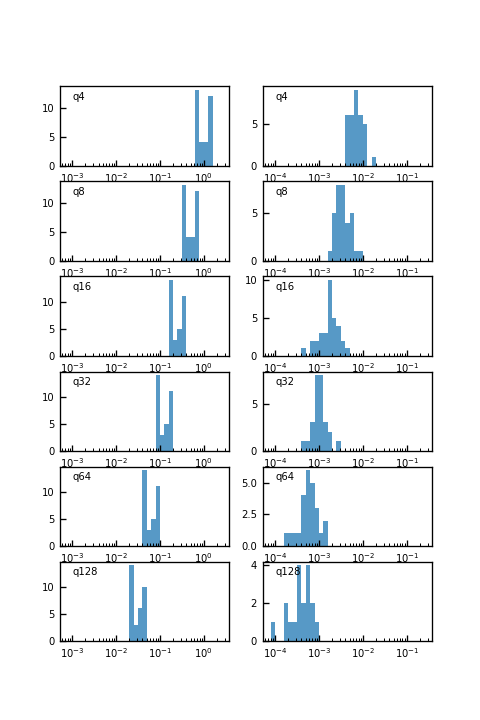
\includegraphics[width=0.95\textwidth]{figure/compression_metric_v2.png}
%        \label{fig:sub1}
    \end{minipage}
    \begin{minipage}{.49\textwidth}
        \centering
        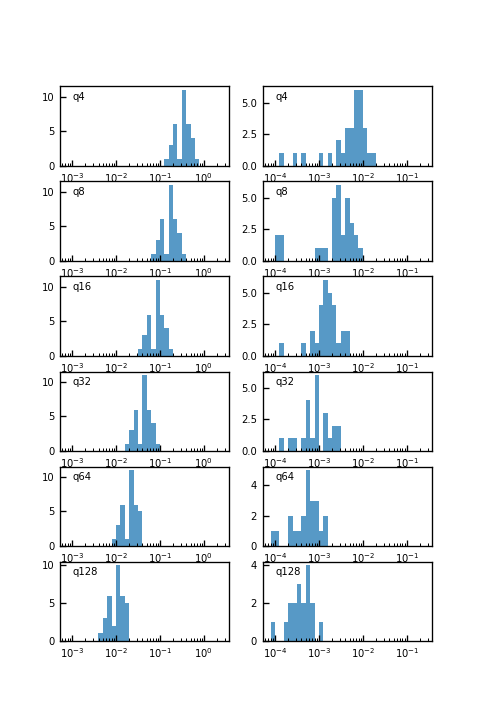
\includegraphics[width=0.95\textwidth]{figure/compression_metric_v2w.png}
%        \label{fig:sub2}
    \end{minipage}
\caption{Histograms showing image level statistics with respect to the original compressed image.
(left two panels) are histograms showing the RMS of the difference between the quantized and original images, 
and the fractional increase in the noise with respect to the original images.  The (right two panels) are the
same analysis but carried out for the weight planes.}
\label{image_difference}
\end{figure}


\clearpage

\subsection{Composite Image Benchmarks}

Beside the individual images, the current tests construct a coadded patch.  
To be clear, this should not be mistaken for constructing, a coadded patch, 
then quantizing, then repeating the previous analysis.  Here the focus is to
understand how properties of the coadd images change when they are constructed
using quantized image products. 

To do this we compare coadd images constructed from the original, 
never-quantized images with coadd images constructed from the quantized images.
In the current limited test, only two coadded images were produced (a single patch 
with two bands) thus the we have only two samples to examine. 
The comparison is further hampered both because the depth of these coadd images 
is shallow (there are only 5 or 6 visits being combined per coadd compared to 100's 
or even 1000's that can be expected from LSST) and to complicate matters further,
the images are no longer in counts (they have been scaled based on a photometric
calibration) and an outlier rejection algorithm is active within the pipeline. 

With these caveats in mind, the comparison at the image level is similar to that made for 
the individual images except that a a constraint has been added to 
remove locations where the clipping algorithm has systematically rejected one of the images.
In the test set there were of order a few such regions per coadd image, overall they were
comprised of a few 10,000's of pixels at q=4 dropping to ~1,000 pixels at q=64).

% Currently that rejection algorithn looks for 20-sigma outliers in the difference between quantized and unquantized (using clipped median and std-deviation) 

The results from the two available samples are summarized in Table~\ref{tab_agg_image_stat}.
The RMS in the coadd image does not vary substantially with the quantization factor.  However, 
when the difference between the coadds constructed from unquantized and quantized images are 
considered the residual is comprised of a roughly Gaussian distribution but with an underlying 
broader distribution that has roughly 10 times the width but 100-1000 times less amplitude.  
In Table~\ref{tab_agg_image_stat} we summarize the width/extent by tracking the min and max differences 
seen in the image/weight planes.

\begin{table}
\caption{Differences in Coadd Images Constructed from Quantized Images}
\centering
\begin{tabular}[]{c|rrr|rrr}
\hline
          &  \multicolumn{3}{c}{Science Plane} & \multicolumn{3}{c}{Weight Plane} \\
 q        &  std($I_{\rm diff}$) & min($I_{\rm diff}$) & max($I_{\rm diff}$) & std($W_{\rm diff}$) & min($W_{\rm diff}$) & max($W_{\rm diff}$) \\
\hline
\multicolumn{7}{c}{Sample 1: HSC-R coadd ($I_{RMS}=0.134$, $W_{RMS}=0.0037$)}  \\
\hline
  4    &  1.3$\times 10^{-2}$ & -1.1$\times 10^{-1}$ & 9.0$\times 10^{-2}$ &  3.8$\times 10^{-5}$ & -5.7$\times 10^{-4}$ & 5.7$\times 10^{-4}$ \\ 
  8    &  6.6$\times 10^{-3}$ & -5.3$\times 10^{-2}$ & 4.2$\times 10^{-2}$ &  1.9$\times 10^{-5}$ & -2.8$\times 10^{-4}$ & 2.8$\times 10^{-4}$ \\
  16   &  3.3$\times 10^{-3}$ & -2.4$\times 10^{-2}$ & 2.1$\times 10^{-2}$ &  1.0$\times 10^{-5}$ & -1.4$\times 10^{-4}$ & 1.4$\times 10^{-4}$ \\
  32   &  1.7$\times 10^{-3}$ & -1.4$\times 10^{-2}$ & 1.4$\times 10^{-2}$ &  5.0$\times 10^{-6}$ & -7.1$\times 10^{-5}$ & 7.1$\times 10^{-5}$ \\
  64   &  8.3$\times 10^{-4}$ & -6.5$\times 10^{-3}$ & 5.6$\times 10^{-3}$ &  2.0$\times 10^{-6}$ & -3.6$\times 10^{-5}$ & 3.6$\times 10^{-5}$ \\
  128  &  4.1$\times 10^{-4}$ & -3.4$\times 10^{-3}$ & 3.4$\times 10^{-3}$ &  1.0$\times 10^{-6}$ & -1.8$\times 10^{-5}$ & 1.8$\times 10^{-5}$ \\
\hline 
\multicolumn{7}{c}{Sample 2: HSC-I coadd ($I_{RMS}=0.232$, $W_{RMS}=0.0076$)}  \\
\hline
  4    &  2.3$\times 10^{-2}$ & -1.7$\times 10^{-1}$ & 1.7$\times 10^{-1}$ &  8.0$\times 10^{-5}$ & -1.1$\times 10^{-3}$ & 1.1$\times 10^{-3}$ \\
  8    &  1.2$\times 10^{-2}$ & -8.9$\times 10^{-2}$ & 8.4$\times 10^{-2}$ &  4.0$\times 10^{-5}$ & -5.6$\times 10^{-4}$ & 5.6$\times 10^{-4}$ \\
  16   &  5.9$\times 10^{-3}$ & -4.3$\times 10^{-2}$ & 4.6$\times 10^{-2}$ &  2.0$\times 10^{-5}$ & -2.8$\times 10^{-4}$ & 2.8$\times 10^{-4}$ \\
  32   &  3.1$\times 10^{-3}$ & -2.5$\times 10^{-2}$ & 2.5$\times 10^{-2}$ &  1.0$\times 10^{-5}$ & -1.4$\times 10^{-4}$ & 1.4$\times 10^{-4}$ \\
  64   &  1.8$\times 10^{-3}$ & -1.8$\times 10^{-2}$ & 1.7$\times 10^{-2}$ &  5.0$\times 10^{-6}$ & -7.0$\times 10^{-5}$ & 7.0$\times 10^{-5}$ \\
  128  &  7.3$\times 10^{-4}$ & -5.9$\times 10^{-3}$ & 5.2$\times 10^{-3}$ &  2.0$\times 10^{-6}$ & -3.5$\times 10^{-5}$ & 3.5$\times 10^{-5}$ \\
\hline
\end{tabular}
\label{tab_agg_image_stat}
\end{table}

%\clearpage

\subsection{Catalog/Measurement benchmarks}

Here we outline the comparison of measurements made on individual ccd-visit images with and without 
quantization applied.  Currently four types of measurements are considered: aperture photometry, 
PSF photometry, centroids, and shapes.  In each case the comparison is made by using forced 
photometry based on the COADD catalogs from the {\it ci\_hsc} run without quantization.
An astrometric match is made between the catalog from the never-quantized images to each of the
catalogs from the quantized images with a 1\arcsec\ match radius (with the nearest source being
considered the match).  The results from multiple CCDs are accumulated into a single plot in order
to obtain statistics at the bright end.

Figures~\ref{plot_se_flux} show comparisons for flux measurements for aperture photometry 
and PSF fitting.  The aperture photometry measurements {\it base\_CircularApertureFlux\_6\_0} 
use a 6 pixel radius circular aperture while the PSF fitting measurements are the
{\it base\_PsfFlux\_flux} measurements.  Note that in these plots no star-galaxy classifier 
was used to subselect stellar/point-source measurements.

The top two panels in each set show the total number of objects per flux bin, followed by a plot 
showing the flux uncertainty as a function of flux from the never-quantized image.  Beneath these 
are plotted the difference between the measurements from the quantized images and the never-quantized 
images with subsequent plots using an increasing level of quantization.  These difference 
plots are shown in units of $\sigma_{\rm F_0}$ (i.e. each difference measurement is scaled by the
uncertainty in the flux measured in the unquantized image).  Overplotted are histograms showing the 
difference level that encompasses 50, 75, 90, and 99\% of the measurements/objects as a function 
of flux bin.  In Table~\ref{tab_se_flux_diff} we report the limiting difference that encompasses
90\% of objects flux measurements for each quantization factor used in this investigation (the cyan
histograms in Figure~\ref{plot_se_flux}).  From Table~\ref{tab_se_flux_diff} it can be seen
that for $q=32$, 90\% of all PSF flux measurements differ by less than 0.1$\sigma$ for objects 
with S/N=3 or higher.   Similarly, 90\% of all aperture flux measurements differ by less than 0.1$\sigma$
for objects with S/N=5 or higher.

Two other avenues have been attempted in looking at these measurements.  The first was to examine the 
uncertainties.  While the uncertainties do change for individual flux measurements on the quantized 
images, there is no evidence that they systematically increase due to the quantization.  The second was
an attempt to examine whether sources were lost/created due to the quantization.  This was not possible
in the case of this study, the measurements were made using forced photometry so the loss/gain of a 
source is directly tied to the detection on the coadd images (which is deeper than
the individual images.

\begin{figure}[t]
\centering
    \begin{minipage}{.49\textwidth}
        \centering
        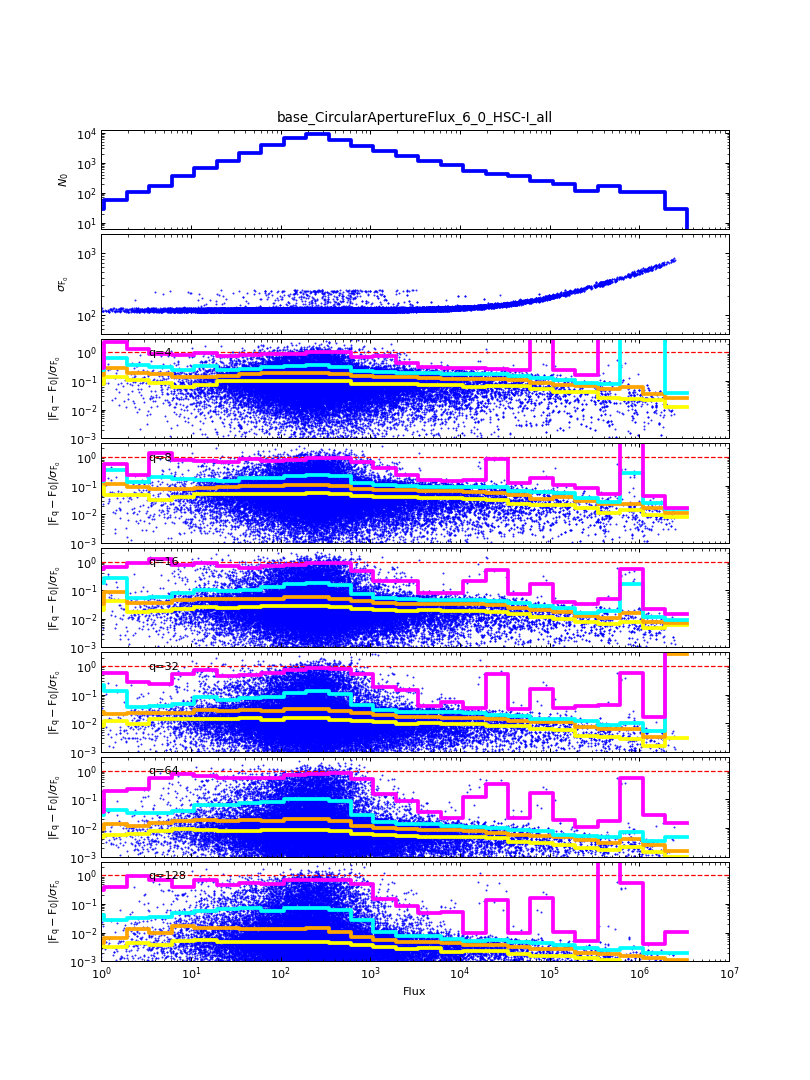
\includegraphics[width=1.0\textwidth]{figure/rplot_all_base_CircularApertureFlux_6_0_HSC-I.png}
%        \label{fig:sub1}
    \end{minipage}
    \begin{minipage}{.49\textwidth}
        \centering
        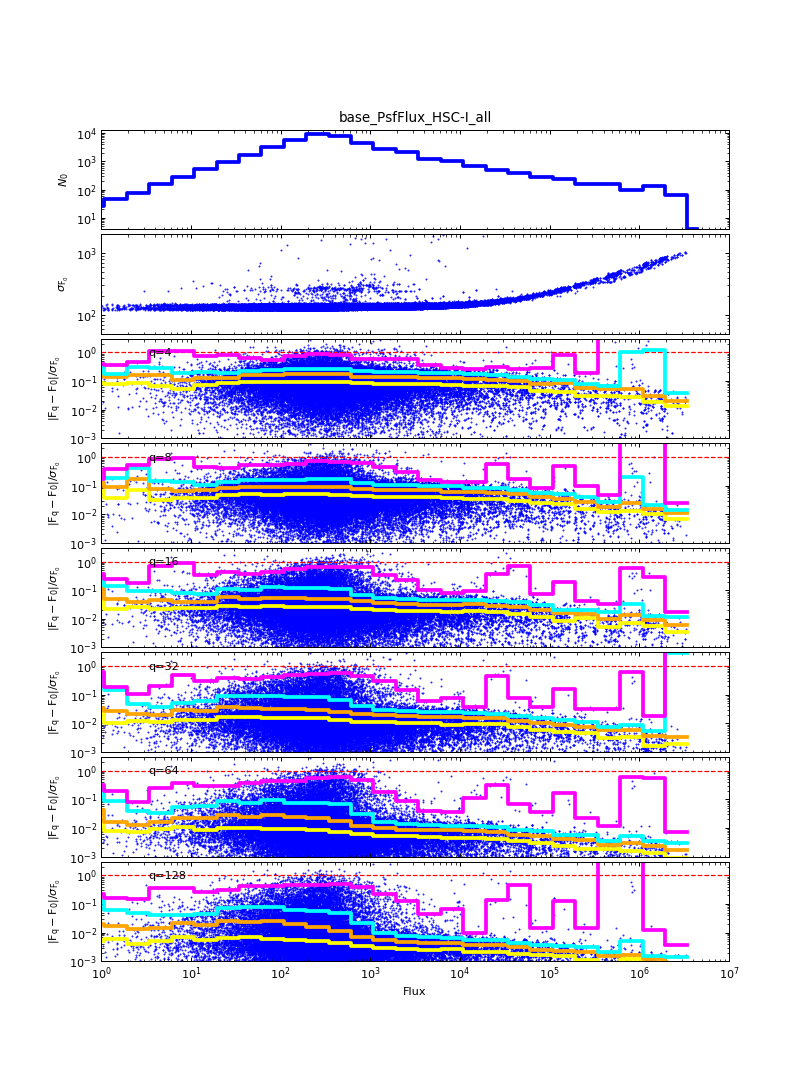
\includegraphics[width=1.0\textwidth]{figure/rplot_all_base_PsfFlux_HSC-I.png}
%        \label{fig:sub2}
    \end{minipage}
\caption{Comparison of aperture (left) and PSF photometry (right) measurements resulting from forced photometry 
on individual images with and without quantization/compression.  The top panel in each shows the distribution 
of objects as a function of their flux measured in the original image(s).  The second plots show measure uncertainties 
for those flux measurements.  The panels below show the difference between the flux measurements made on the
unquantized and quantized images divided by the uncertainty in the quantized images (in units of $\sigma_{\rm F_0}$.  
A dashed horizontal red line shows the 1$\sigma$ difference level for reference.  The lower panels are for 
measurements from the images with progressively higher quantization factors (less loss).
The histograms in each panel show the difference level at which 50, 75, 90 and 90\% of the objects are found.}
\label{plot_se_flux}
\end{figure}

\begin{table}[ht]
\caption{Maximum Flux Difference (in units of $\sigma_{\rm F_0}$) for 90\% of Objects}
\centering
\begin{tabular}[]{c|rrrr|rrrr}
\hline
     &  \multicolumn{4}{c}{PSF Flux}  & \multicolumn{4}{c}{Aperture Flux} \\
 q   &  S/N=3 & S/N=5 & S/N=10 & S/N=100 & S/N=3 & S/N=5 & S/N=10 & S/N=100  \\
\hline
   4 &  0.266 & 0.234 & 0.208  & 0.171 &   0.332 & 0.269 & 0.208 & 0.171 \\
   8 &  0.161 & 0.136 & 0.110  & 0.087 &   0.220 & 0.170 & 0.113 & 0.089 \\
  16 &  0.106 & 0.078 & 0.056  & 0.044 &   0.163 & 0.113 & 0.058 & 0.044 \\
  32 &  0.074 & 0.050 & 0.031  & 0.022 &   0.117 & 0.068 & 0.033 & 0.022 \\
  64 &  0.067 & 0.043 & 0.018  & 0.011 &   0.097 & 0.064 & 0.019 & 0.011 \\
 128 &  0.049 & 0.027 & 0.011  & 0.006 &   0.067 & 0.042 & 0.014 & 0.006 \\
\hline
\end{tabular}
\label{tab_se_flux_diff}
\end{table}


Similar to the flux measurements, Figure~\ref{plot_cen_shape} shows comparisons of centroid
and shape measurements (left and right panels, respectively) as a function of signal-to-noise
(S/N) in the unquantized images.  For the centroids we use the {\it base\_SdssCentroid\_x} (x), and 
{\it base\_SdssCentroid\_y} (y), to compute the linear offset 
$X_q-X_0 = \sqrt{ (x_q-x_0)^2 + (y_q-y_0)^2}$ between the measurements
made in the quantized and unquantized images.  Note that the version of forced photometry that is 
deployed in this test does not flag poor and low signal-to-noise measurements so those measurements 
pollute/inflate the distributions show in the low signal-to-noise portion of the centroid plots 
in Figure~\ref{plot_cen_shape}.

In order to investigate the impact of quantization on shapes, we use the {\it base\_SdssShape\_xx}, 
{\it base\_SdssShape\_yy}, and {\it base\_SdssShape\_xy} measurements to form a shape measurement, 
$S$, where $S=(I_{xx} I_{yy} - I_{xy}^2)^{1/4}$.
Assuming that those 2nd moment measurements are not strongly correlated, we also define
the uncertainty in $S$ as 
$\sigma_S^2 = (\frac{\partial S}{\partial I_{xx}})^2 \sigma_{I_{xx}}^2 + 
(\frac{\partial S}{\partial I_{yy}})^2 \sigma_{I_{yy}}^2 + 
(\frac{\partial S}{\partial I_{xy}})^2 \sigma_{I_{xy}}^2$, and use the associated uncertainties
to estimate $\sigma_S$.  Figure~\ref{plot_cen_shape} shows these measurements and makes a comparison
of the quantized measurements to those found with the unquantized images.  Measurements with 
{\it base\_SdssShape\_flag} have been excluded.

In Table~\ref{tab_se_cen_shape_diff} we summarize the limiting difference that encompasses 90\% of 
objects centroid and shape differences (the cyan histograms in Figure~\ref{plot_cen_shape}).  
From Table~\ref{tab_se_cen_shape_diff} it can be seen
that for $q=16$, 90\% of all centroid measurements from sources with S/N=10 or higher differed by less
than 0.1 pixel.  Similarly, at $q=16$, shapes/sizes differ by less than 0.1 pixel for S/N=5 or higher.

\begin{figure}[t]
\centering
    \begin{minipage}{.49\textwidth}
        \centering
        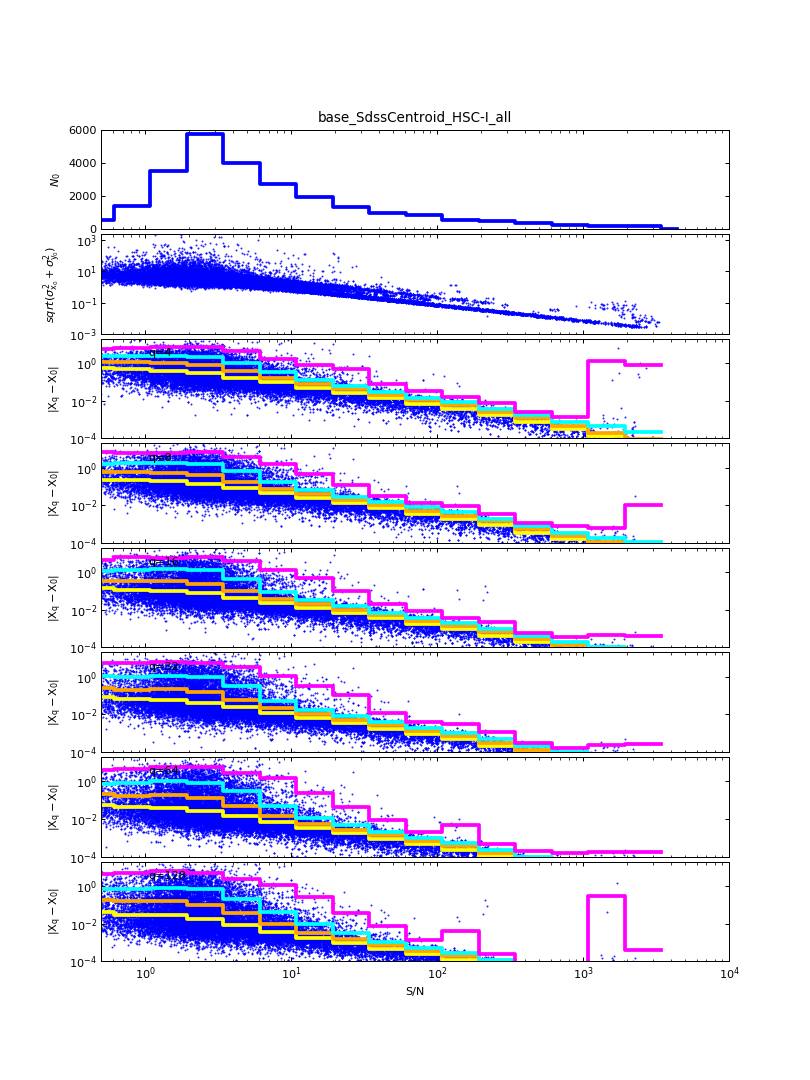
\includegraphics[width=1.0\textwidth]{figure/rplot_all_base_SdssCentroid_HSC-I.png}
%        \label{fig:sub1}
    \end{minipage}
    \begin{minipage}{.49\textwidth}
        \centering
        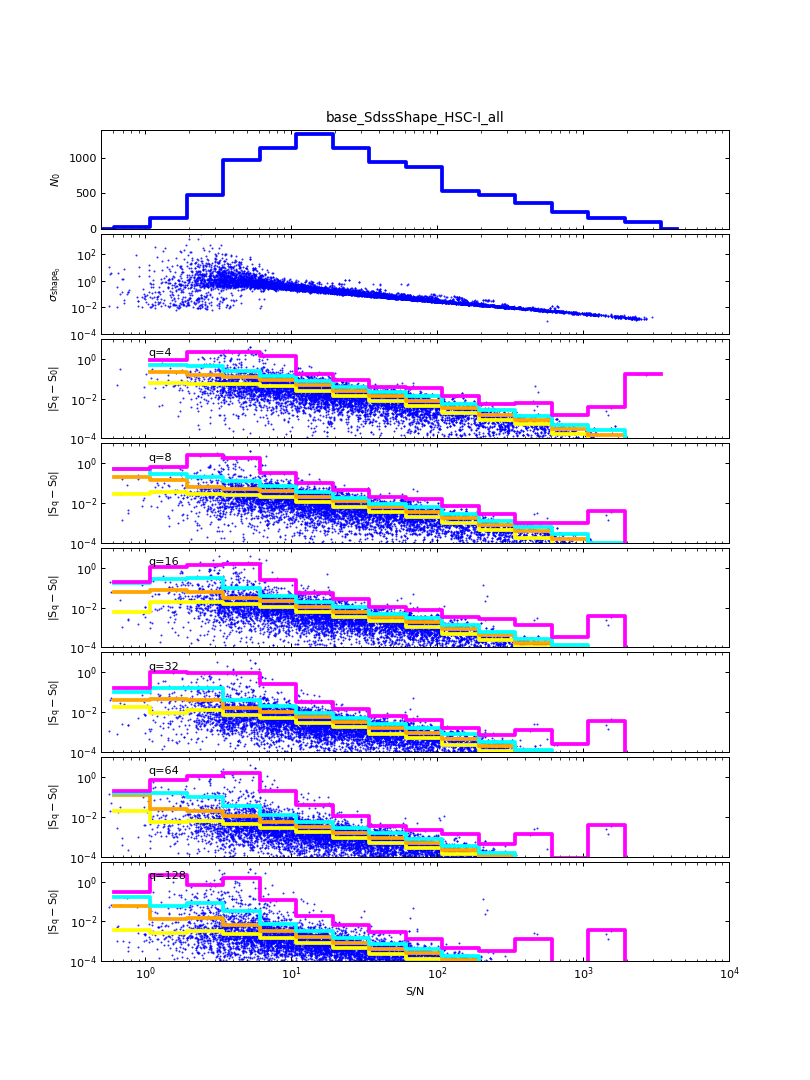
\includegraphics[width=1.0\textwidth]{figure/rplot_all_base_SdssShape_HSC-I.png}
%        \label{fig:sub2}
    \end{minipage}
\caption{Similar to Figures~\ref{plot_se_flux} but for centroid (left) and shape (right) measurements as function 
of the signal-to-noise ratio of the unquantized measurements.  The differences in the lower panels 
are in units of pixel offset and pixel radius for the centroid and shape measurements, respectively.}
\label{plot_cen_shape}
\end{figure}

\begin{table}
\caption{Maximum Centroid and Shape Difference for 90\% of Objects}
\centering
\begin{tabular}[]{c|rrrr|rrrr}
\hline
     &  \multicolumn{4}{c}{Centroid}  & \multicolumn{4}{c}{Shape} \\
 q   &  S/N=3 & S/N=5 & S/N=10 & S/N=100 & S/N=3 & S/N=5 & S/N=10 & S/N=100  \\
\hline
   4 & 1.791 & 0.898 & 0.269  & 0.013 &  0.370 & 0.231 & 0.112  & 0.010 \\
   8 & 1.364 & 0.590 & 0.129  & 0.007 &  0.183 & 0.118 & 0.058  & 0.005 \\
  16 & 1.063 & 0.375 & 0.066  & 0.003 &  0.255 & 0.083 & 0.030  & 0.002 \\
  32 & 0.778 & 0.276 & 0.039  & 0.002 &  0.136 & 0.039 & 0.016  & 0.001 \\
  64 & 0.704 & 0.258 & 0.036  & 0.001 &  0.080 & 0.030 & 0.009  & 0.001 \\
 128 & 0.540 & 0.169 & 0.029  & $<$0.001 &  0.066 & 0.029 & 0.006  & $<$0.001 \\
\hline
\end{tabular}
\label{tab_se_cen_shape_diff}
\end{table}



\clearpage

\subsection{Catalog/Measurement from COADD images constructed from quantized PVI images}

Similar to the comparisons made for the individual images, we compare the catalog measurements from the coadded patch
that was constructed from the never-quantized and the quantized PVI images.  The same four quantities were examined 
(aperture flux, PSF flux, centroid, and shape).  Figures~\ref{plot_coadd_flux} and \ref{plot_coadd_cen_shape} show
the results of that comparison and Tables~\ref{tab_coadd_flux_diff} and \ref{tab_coadd_cen_shape_diff} report the 
limiting difference that encompasses 90\% of objects measurements.

Based on the results in Table~\ref{tab_coadd_flux_diff} it can be seen that for coadds constructed from images 
with $q=64$, 90\% of all PSF and aperture flux measurements differ by less than 0.1$\sigma$ for objects 
with S/N=10 or higher.  While this does suggest that lower quantization factors (and higher compression factors)
might be less desirable, it should be noted that these coadds, comprised of only a few visit images, are extreme 
cases compared to those that would result from the LSST survey (with many 100's of images per band at each location
in the survey footprint).  Clearly a more realistic test should be implemented.

The difference measured in the centroids and shapes show a somewhat different trend.  Considering the 
vales in Table~\ref{tab_coadd_cen_shape_diff} the quantization also seems to make modest differences on 
the centroid measurements but the shapes show much smaller changes.  For coadds constructed with q=64, 90\% 
of objects with S/N=10 are recovered with differences of less than 0.1 pixels (whereas the single-image
measurements reached the same benchmark for q=16).  On the other hand, the shape measurements for objects with
S/N=5 match those in the coadds constructed from un-quantized images for q=16 (similar to what was found 
for the single-image measurements).

Unlike the measurements on the individual images (which used a forced photometry algorithm), object detection 
was performed independently on the COADD images in each test.  Therefore, we can also characterize the 
loss/creation of sources for the COADDs images constructed from quantized PVI images.  
In Table~\ref{tab_coadd_lost_found} we summarize the numbers of objects that were detected on the original COADD 
images but were not detected on the COADDs built from quantized PVIs (the ``lost'' sources)
as well as the converse, ``new'' sources (identified on the COADDs constructed from the quantized PVIs).  We tabulate
separately, numbers of sources without considering whether the objects were flagged and then repeat the exercise 
considering only unflagged sources.  We also present the distribution of the unflagged sources
that were lost and created as a function of their signal-to-noise (based on the PSF flux/uncertainty measurements)
in Figure~\ref{plot_coadd_lost_found}.  These show that only faint sources are affected with only minimal changes 
occurring with S/N > 10.  We again caution that this analysis is based on a test set that is constructed from a few 
rather than 100's of images that would be used in LSST COADDs.  We also note that a cross check was made where we
examined the lost/new source locations on the images and suspect that the signal-to-noise measurements may be
systematic over-estimates.



\begin{figure}[t]
\centering
    \begin{minipage}{.49\textwidth}
        \centering
        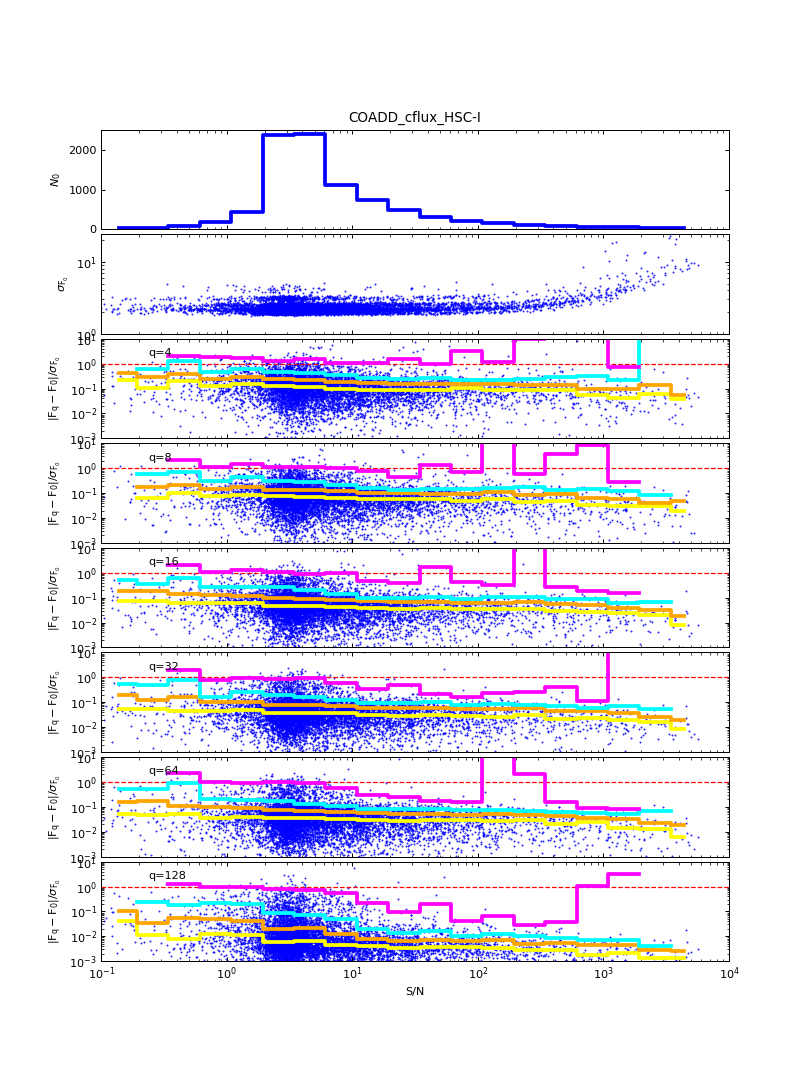
\includegraphics[width=1.0\textwidth]{figure/plot_coadd_cflux_HSC-I.png}
%        \label{fig:sub1}
    \end{minipage}
    \begin{minipage}{.49\textwidth}
        \centering
        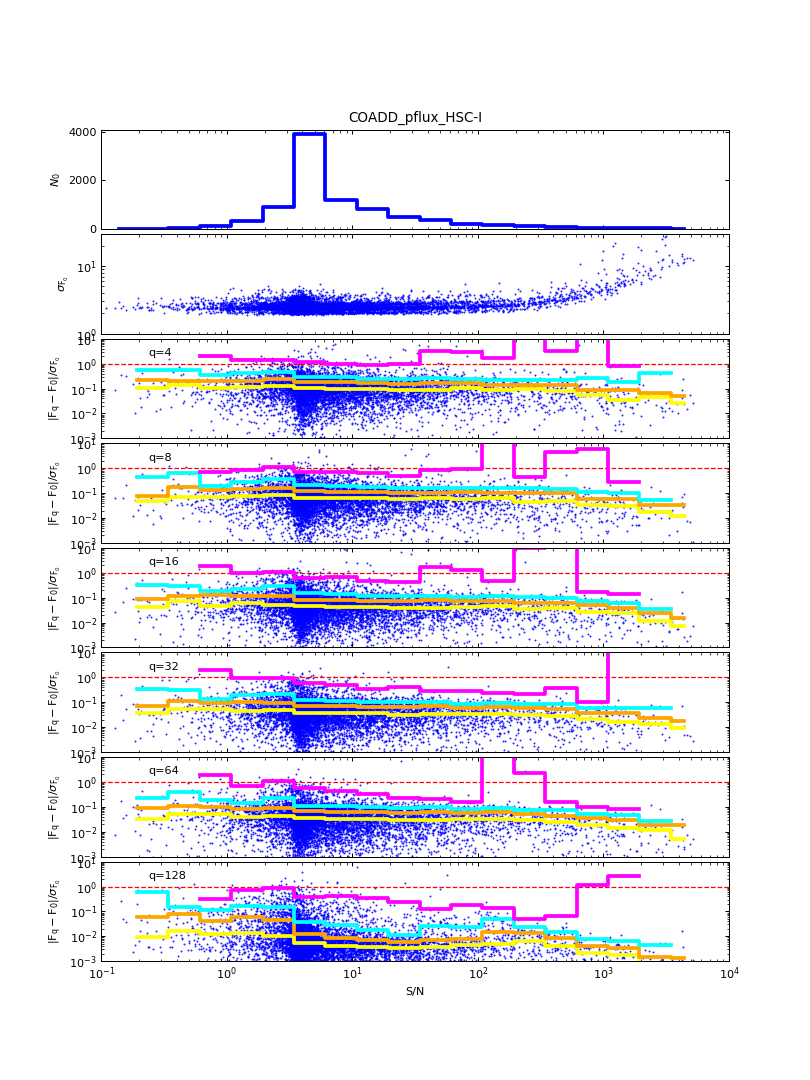
\includegraphics[width=1.0\textwidth]{figure/plot_coadd_pflux_HSC-I.png}
%        \label{fig:sub2}
    \end{minipage}
\caption{Similar to Figure~\ref{plot_se_flux} but for measurements made on the coadd image.}
\label{plot_coadd_flux}
\end{figure}


\begin{figure}[t]
\centering
    \begin{minipage}{.49\textwidth}
        \centering
        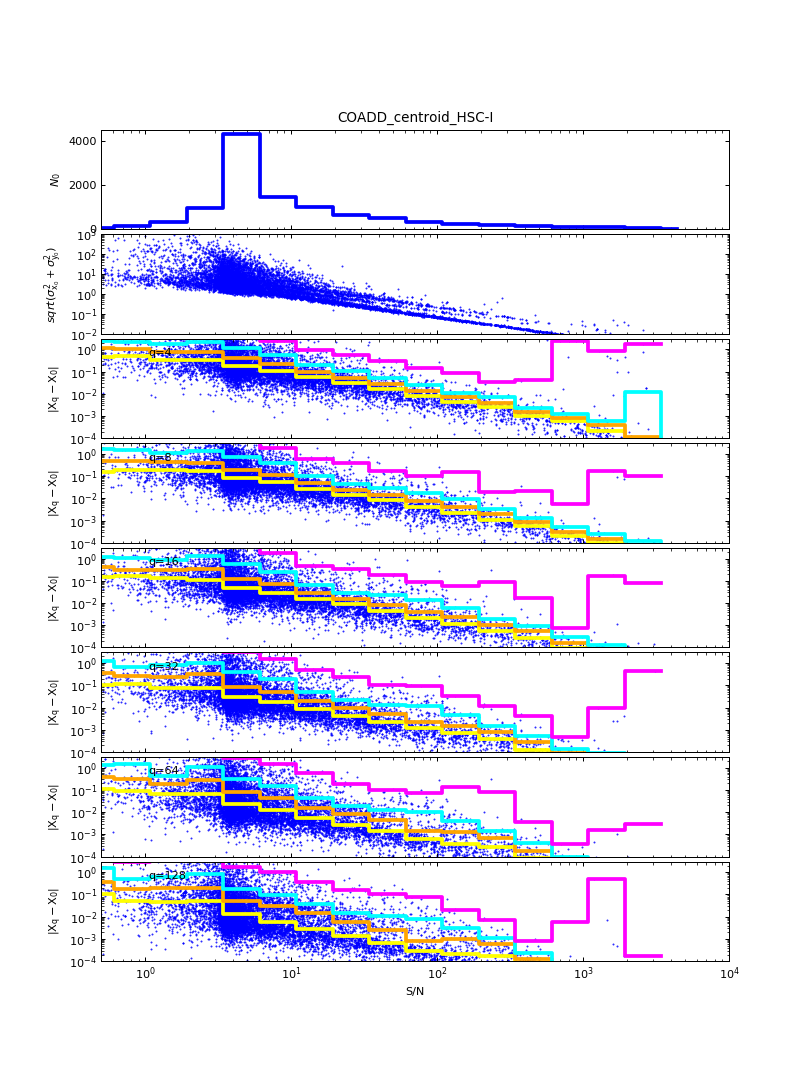
\includegraphics[width=1.0\textwidth]{figure/plot_coadd_centroid_HSC-I.png}
%        \label{fig:sub1}
    \end{minipage}
    \begin{minipage}{.49\textwidth}
        \centering
        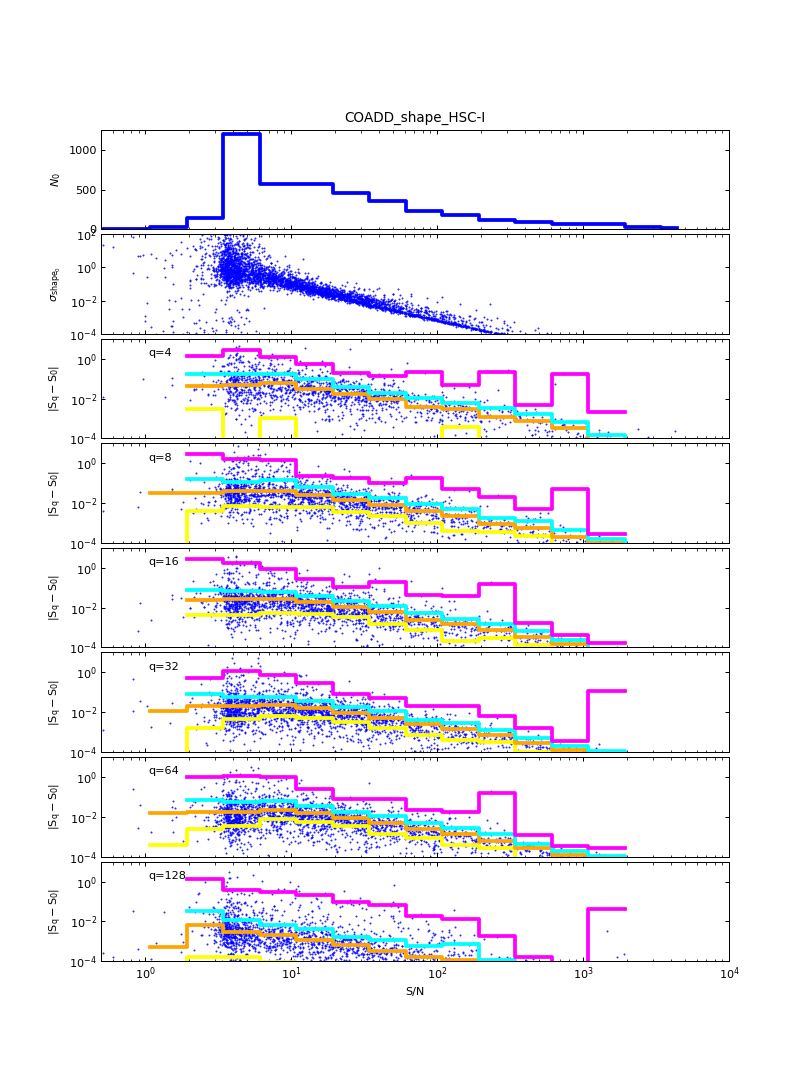
\includegraphics[width=1.0\textwidth]{figure/plot_coadd_shape_HSC-I.png}
%        \label{fig:sub2}
    \end{minipage}
\caption{Similar to Figure~\ref{plot_cen_shape} but for measurements made on the coadd image.}
\label{plot_coadd_cen_shape}
\end{figure}


\begin{table}[hb]
\caption{Maximum Flux Difference (in units of $\sigma_{\rm F_0}$) for 90\% of COADD Objects}
\centering
\begin{tabular}[]{c|rrrr|rrrr}
\hline
     &  \multicolumn{4}{c}{PSF Flux}  & \multicolumn{4}{c}{Aperture Flux} \\
 q   &  S/N=3 & S/N=5 & S/N=10 & S/N=100 & S/N=3 & S/N=5 & S/N=10 & S/N=100  \\
\hline
   4 & 0.405 & 0.297 & 0.274 &  0.233   &  0.453 & 0.413 & 0.307 &  0.216 \\
   8 & 0.333 & 0.203 & 0.189 &  0.158   &  0.296 & 0.278 & 0.198 &  0.154 \\
  16 & 0.252 & 0.149 & 0.129 &  0.113   &  0.246 & 0.194 & 0.128 &  0.095 \\
  32 & 0.184 & 0.120 & 0.111 &  0.089   &  0.181 & 0.151 & 0.110 &  0.081 \\
  64 & 0.198 & 0.111 & 0.103 &  0.084   &  0.163 & 0.129 & 0.099 &  0.075 \\
 128 & 0.120 & 0.036 & 0.024 &  0.033   &  0.085 & 0.069 & 0.038 &  0.011 \\
\hline
\end{tabular}
\label{tab_coadd_flux_diff}
\end{table}



\begin{table}
\caption{Maximum Centroid and Shape Difference for 90\% of COADD Objects}
\centering
\begin{tabular}[]{c|rrrr|rrrr}
\hline
     &  \multicolumn{4}{c}{Centroid}  & \multicolumn{4}{c}{Shape} \\
 q   &  S/N=3 & S/N=5 & S/N=10 & S/N=100 & S/N=3 & S/N=5 & S/N=10 & S/N=100  \\
\hline
   4 & 1.926 & 1.109 & 0.460 &  0.025   &  0.167 & 0.175 & 0.146 &  0.009 \\
   8 & 1.296 & 0.724 & 0.309 &  0.025   &  0.151 & 0.122 & 0.121 &  0.007 \\
  16 & 1.208 & 0.525 & 0.219 &  0.018   &  0.075 & 0.066 & 0.056 &  0.004 \\
  32 & 0.898 & 0.378 & 0.156 &  0.014   &  0.076 & 0.057 & 0.052 &  0.004 \\
  64 & 0.920 & 0.329 & 0.125 &  0.013   &  0.067 & 0.056 & 0.051 &  0.004 \\
 128 & 0.730 & 0.163 & 0.084 &  0.009   &  0.028 & 0.011 & 0.006 &  0.001 \\
\hline
\end{tabular}
\label{tab_coadd_cen_shape_diff}
\end{table}


\begin{table}
\caption{Lost and Created Sources in COADD}
\centering
\begin{tabular}[]{cr|rr|rr}
\hline
     &                  & \multicolumn{2}{c}{w/ Flagged}  & \multicolumn{2}{c}{w/o Flagged} \\
 q   & N$_{\rm object}$ & Lost & Created                  & Lost & Created  \\
\hline
   0 & 13851 &      &      &      &      \\
   4 & 15144 & 1728 & 2897 & 1248 &  871 \\
   8 & 13170 & 1717 & 1001 &  964 &  528 \\
  16 & 13866 &  902 &  889 &  735 &  434 \\
  32 & 13924 &  647 &  698 &  540 &  326 \\
  64 & 13872 &  636 &  632 &  541 &  330 \\
 128 & 14508 &  374 &  987 &  149 &  223 \\
\hline
\end{tabular}
\label{tab_coadd_lost_found}
\end{table}


\begin{figure}[t]
\centering
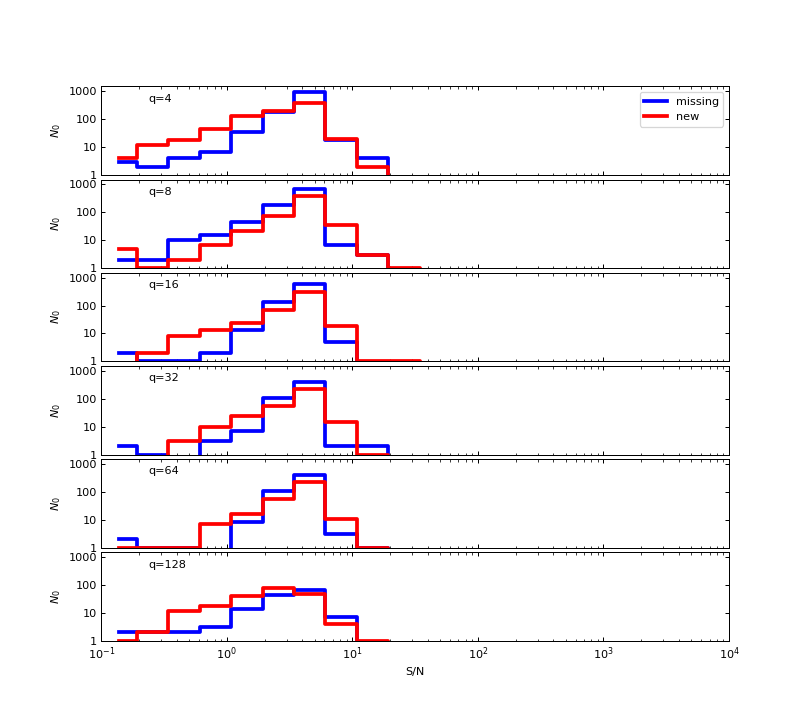
\includegraphics[width=0.75\textwidth]{figure/plot_coadd_missing_HSC-I.png}
\caption{Distribution of S/N of objects that are lost/new when detection is run on COADDs constructed from 
quantized images.}
\label{plot_coadd_lost_found}
\end{figure}



% \subsection{Lost Objects}


\clearpage

\section{Compression Algorithm benchmarks}

We have applied a variety of existing compression algorithms to the quantized images from this study to 
obtain benchmarks of their efficacy.  The values reported reflect those algorithms' performance when
running under OS X 10.13.2 (macOS High Sierra) on a MacBook Pro with quad 2.9 GHz processors.  A ramdisk
was used for storage to minimize the impact of I/O operations within the test.  

A range of existing algorithms have been benchmarked, including a number which use threading to achieve 
greater speed.  The algorithms considered were:
\begin{enumerate}
\item {\bf gzip:} the standard GNU implementation of Lempel-Ziv (LZ77).
\item {\bf pigz:} a threaded version of gzip.
\item {\bf bzip2:} an implementation of Burrows-Wheeler block sorting (offers the possibility of recovery of undamage block).
\item {\bf pbzip2:} a threaded/parallel implementation of bzip2.
\item {\bf lbzip2:} another threaded/parallel implementation of bzip2.
\item {\bf lz4:} a "typically faster" implementation of LZ77 (favoring speed over compression ratio). Pushing to higher compression ratios significantly degrades performance.
\item {\bf lzop:} an implementation of LZ77 trading a hit in compression time for an improvement in decompression.  
The performance trade is not apparent for the file size in these tests.
\item {\bf zstd:} Also based on LZ77 and includes a parallel implementation.  In addition there
exist implementations/bindings for a wide variety of languages (including Python).  
\item {\bf zstd$^\star$:} zstd but with use of a pre-computed dictionary to obtain an improvement
in speed and/or compression factor.  Rigorous testing was not possible for this small set but performance
was identical to the untrained algorithm if the full set was used both to train and then obtain benchmarks.
\item {\bf xz:} Based on the LZMA variant of LZ77.  Good compression factors can be achieved 
but in order to get better performance some tuning will be necessary (see xz$^\prime$ below).
\item {\bf xz$^\prime$:} Used xz with an command line overide of $-$1 to obtain a factor of 10 in performance (speed)
at a modest cost in compression factor. 
\end{enumerate}

The results from benchmark tests are summarized in Tables~\ref{compress_factor}-\ref{timing_decompress}, 
showing compression factor, time to compress per file, and time to decompress per file, respectively.
These times do not include the time to necessary to obtain and apply scale factor used in the quantization.  
Furthermore, the set of files being compressed are nearly identical (98 Mb) and therefore do not provide 
any information about algorithmic performance with respect to file size.  When a parallel implementation
was available the threading was set to use 4 cores.


\begin{table}
\caption{Compression Factor Achieved}
\centering
\begin{tabular}[]{crrrrrrrrrrr}
\hline
 q        &  gzip & pigz & bzip2 & pbzip2 & lbzip2 & lz4 & lzop & zstd & zstd$^\star$ & xz & xz$^\prime$  \\
\hline
 4       &   6.73 &  6.73 &  9.96 &  9.95 &  9.96 &  3.69 &  3.11 &  6.29 &  6.29 & 10.06 &  8.19  \\
 8       &   5.54 &  5.53 &  8.20 &  8.20 &  8.21 &  3.34 &  2.96 &  5.42 &  5.42 &  8.20 &  6.79  \\
 16      &   4.69 &  4.69 &  5.41 &  7.01 &  7.03 &  3.11 &  2.82 &  4.82 &  4.82 &  6.96 &  6.01  \\
 32      &   4.04 &  4.03 &  6.14 &  6.14 &  6.14 &  2.93 &  2.66 &  4.35 &  4.35 &  6.00 &  5.44  \\
 64      &   3.62 &  3.62 &  5.47 &  5.47 &  5.48 &  2.82 &  2.47 &  3.94 &  3.94 &  5.29 &  4.95  \\
 128     &   3.38 &  3.37 &  4.88 &  4.88 &  4.88 &  2.66 &  2.32 &  3.56 &  3.57 &  4.75 &  2.51  \\
 vanilla  &   1.71 &  1.71 &  1.80 &  1.80 &  1.80 &  1.50 &  1.49 &  1.72 &  1.72 &  1.87 &  1.80  \\
\hline
\end{tabular}
\label{compress_factor}
\end{table}


\begin{table}
\caption{Time to Compress per File}
\centering
\begin{tabular}[]{crrrrrrrrrrr}
\hline
 q        &  gzip & pigz & bzip2 & pbzip2 & lbzip2 & lz4 & lzop & zstd & zstd$^\star$ & xz & xz$^\prime$  \\
\hline
  4       &    4.45 &   1.18 &   5.00 &   1.42 &   0.85 &   0.21 &   0.24 &   0.36 &   0.12 &  55.27 &   3.33  \\
  8       &    6.06 &   1.64 &   4.91 &   1.39 &   0.82 &   0.21 &   0.24 &   0.42 &   0.15 &  50.94 &   4.12  \\
 16      &    8.27 &   2.24 &   4.33 &   1.39 &   0.82 &   0.27 &   0.27 &   0.55 &   0.18 &  50.09 &   4.27  \\
 32      &   10.30 &   2.76 &   5.27 &   1.42 &   0.79 &   0.24 &   0.27 &   0.58 &   0.21 &  47.36 &   4.64  \\
 64      &   11.79 &   3.00 &   5.39 &   1.52 &   0.88 &   0.24 &   0.30 &   0.61 &   0.24 &  47.48 &   5.09  \\
 128     &   12.76 &   3.21 &   5.91 &   1.61 &   0.94 &   0.27 &   0.30 &   0.67 &   0.21 &  54.21 &   2.52  \\
 vanilla  &    3.36 &   0.97 &   8.94 &   2.79 &   1.58 &   0.15 &   0.12 &   0.30 &   0.15 &  34.00 &  15.15  \\
\hline
\end{tabular}
\label{timing_compress}
\end{table}

\begin{table}
\caption{Time to Decompress per File}
\centering
\begin{tabular}[]{crrrrrrrrrrr}
\hline
 q        &  gzip & pigz & bzip2 & pbzip2 & lbzip2 & lz4 & lzop & zstd & zstd$^\star$ & xz & xz$^\prime$  \\
\hline
 4       &    0.21 &   0.24 &   2.30 &   1.21 &   1.27 &   0.15 &   0.18 &   0.27 &   0.24 &   0.82 &   1.06  \\
 8       &    0.24 &   0.27 &   2.33 &   1.12 &   1.24 &   0.18 &   0.18 &   0.27 &   0.27 &   0.97 &   1.27  \\
 16      &    0.27 &   0.27 &   2.02 &   1.12 &   1.21 &   0.18 &   0.18 &   0.27 &   0.24 &   1.09 &   1.33  \\
 32      &    0.30 &   0.30 &   2.42 &   1.24 &   1.24 &   0.15 &   0.18 &   0.27 &   0.24 &   1.27 &   1.42  \\
 64      &    0.30 &   0.30 &   2.42 &   1.27 &   1.09 &   0.18 &   0.21 &   0.27 &   0.27 &   1.42 &   1.48  \\
 128     &    0.30 &   0.33 &   2.82 &   1.30 &   1.24 &   0.24 &   0.21 &   0.30 &   0.27 &   1.52 &   0.67  \\
 vanilla  &    0.39 &   0.36 &   4.36 &   1.48 &   1.27 &   0.15 &   0.12 &   0.24 &   0.24 &   3.58 &   3.52  \\
\hline
\end{tabular}
\label{timing_decompress}
\end{table}



\clearpage

\section{Recommendations}

Originally the intent of this investigation was to match these results to requirements within the 
LSST \SRD \citedsp{LPM-17}.  This has proven relatively difficult for many reasons.
First, the \SRD is geared toward instrument/hardware performances, and most requirements are not 
stated with a performance for a source at a specific signal-to-noise.  The guiding principle is
\begin{quote} ...the measurement errors for fundamental quantities, 
such as astrometry, photometry and image size, should not be dominated by algorithmic performance.
\end{quote}
The differences that result when making measurements on the quantized single-epoch images are typically 
much smaller than the associated uncertainties when making the same measurement on the never-quantized
images.  In terms of source flux, at S/N=10 if those differences are adopted as an additional uncertainty, 
90\% of sources would show an increase of less than $\frac{1}{10}$th in their uncertainty when quantization 
is applied.  In addition there is no evidence that the uncertainties of the measurements on the quantized 
images systematically increase.

Below, our recommendations assume:
\begin{itemize}

\item The capability to recompute a reduced-calibrated image product on-the-fly will be 
possible for users that need such.

\item Astronomers have the scientific acumen to understand that measurements and products 
made using lossy-compressed images will not exactly match those made during release production.

\item The tests in this note are inadequate in a couple of respects.  The measurement
algorithms are not those that will be deployed in the LSST Alert and Data Release Processing.
The COADD images/catalogs in the current tests are comprised of a small amount of data
and therefore cover a small area and are comprised of 10 to 100 times fewer images than 
will be the case in the LSST survey.  In order to have a detailed understanding
of the impact of compression a much larger dataset than {\it ci\_hsc} is needed.

\end{itemize}


With these in mind we recommend the following:
\begin{enumerate}
\item {\bf Overall:} A lossy compression can certainly be used by LSST to store products that would 
not otherwise have been available to scientists. Data Release Processing (DRP) PVI images are the 
clearest case where lossy compression should be considered as these products otherwise would not be stored, 
requiring re-computation, or would require a large tape storage infrastructure. 

\item {\bf Quantization Factor:} Most scientific use cases should be satisfied by a quantization 
factor of q=16 or q=32.  Measurements of sources with S/N=10 or greater, made from quantized images 
do not show significant systematic differences from those made on un-quantized data products.  

\item {\bf Algorithm:} The best performing, off-the-shelf candidate for compression is BZIP2 which 
achieves a compression factor of 5-7.  The main drawback to BZIP2 is speed but in trading speed for 
compression factor the use of LZ or ZSTD would roughly double the storage costs.  

\item {\bf When and where to use lossy compression:}  Compression should occur after production
but before archiving.  This ameliorates any risk that compression adversely impacts the ability 
of LSST to meet science requirements.  The availability of compressed products for
users is meant to allow followup investigations to proceed without an explicit need for reprocessing.  

\item {\bf Other Products:} Within the data storage model there are a few other products that 
might be considered as candidates for lossy compression.  These are: the Data Release Processing
(DRP) COADD images, the Alert Processing (AP) templates, and the 60-day store of PVI images from 
the AP pipeline for PreCovery of transients.  The realized benefit of storing any of these with 
lossy compression is 100's of times smaller than the DRP PVI images.  Moreover, if lossy compression 
were used for any of these AP data types, there would be a direct impact on the production results.  
Therefore we do NOT recommend use of lossy compression without a demonstration that its use would 
not prevent reaching survey requirements.  To do so requires a detailed test with working versions
of the pipelines and real? LSST data. 

\item {\bf Verification:} The current tests are not realized within the LSST framework or QA effort.
They costly to make as they require production to be repeated for each level of quantization.  
It is recommended that a means to implement tests similar to those detailed here be considered 
so that as the pipelines and LSST measurement algorithms mature real tests on real data can verify
and set the quantization value appropriately.

\item {\bf User Interfaces:} If lossy compression is used there will need to be a decision whether it
should be applied on the image pixels only or at the file level.  The former has the advantage that 
header information could be accessible without decompressing but means that common tools (especially
those developed external to LSST) would need additions.  The latter choice would alleviate that problem
but would place the onus on users (and pipelines) to have the ability to recognize and decompress 
such products before they could be used.

\end{enumerate}


\section{WG Membership}

Membership of roughly four people is optimal and should include persons familiar 
with weak-lensing and difference imaging concerns.
The proposed membership is:

\begin{itemize}
    \item Robert Gruendl (NCSA; \textbf{Chair}),
    \item Paul Price (Princeton),
    \item Bob Armstrong (Princeton),
    \item Krzysztof Findeisen (UW; replacing John Parejko),
    \item Sophie Reed (Princeton),
    \item Eric Morganson (DES/NCSA; observer)
    \item Ben Emmons (EPO Tucson; observer)
\end{itemize}

